\documentclass{article}

\usepackage{amsmath}
\usepackage{amsfonts}
\usepackage{amssymb}
\usepackage{graphicx}
\usepackage[dvipsnames]{xcolor}
\usepackage[margin=0.5in]{geometry}
\usepackage[hidelinks]{hyperref}
\usepackage{enumitem}

\usepackage{array}

\graphicspath{{.}{./img/}}

\let\oldemptyset\emptyset
\let\emptyset\varnothing
\newcommand{\Ti}{\textcolor{red}{ti}}
\newcommand{\It}{\textcolor{blue}{it}}
\newcommand{\LC}[3]{\mathsf{LC}(#1,\, #2,\, #3)}
\newcommand{\frequent}[1]{\textcolor{OliveGreen}{#1}}
\newcommand{\infrequent}[1]{\textcolor{BrickRed}{#1}}
\newcommand{\intersects}[1]{\textcolor{BlueViolet}{#1}}
\usepackage{tikz-qtree}

\usepackage{environ}
\NewEnviron{centerframebox}{\begin{center}\fbox{\parbox{0.92\textwidth}{\BODY}}\end{center}}

\title{Algorithms for Data Science \\ Exercise Sheet 4}
\author{
  Vladislav Imashev \\ \href{mailto:s05vimas@uni-bonn.de}{s05vimas@uni-bonn.de} \and
  AAAAAAAAAA AAAAAAA \\ \href{mailto:AAAAAAAAAAAAAAAAAAAA}{AAAAAAAAAAAAAAAAAAAA} \and
  German Mikhelson \\ \href{mailto:s17gmikh@uni-bonn.de}{s17gmikh@uni-bonn.de} \and
  Aleksandra Volynets \\ \href{mailto:s02avoly@uni-bonn.de}{s02avoly@uni-bonn.de} \and
  Nikita Morev \\ \href{mailto:s99nmore@uni-bonn.de}{s99nmore@uni-bonn.de}
}

\begin{document}
  \maketitle

  \setcounter{section}{4}
  \subsection{Closed itemsets}
  \begin{centerframebox}
    Let $\mathcal{D}$ be a transaction database over $I$ and let $X \subseteq I$. Is
    it true that $X$ is closed if and only if $\mathcal{D}[X \cup \{i\}] \subsetneq \mathcal{D}[X]$ holds for all
    $i \in I \setminus X$? Prove your answer.
  \end{centerframebox}

  $\Rightarrow$: Let $i \in I: \mathcal{D}[X \cup {i}] = \mathcal{D}[X]$ therefore, $i$ had no effect on the \textit{support} when adding it to $X$, and this contradicts the property that
  \[X\text{ is closed} \iff |\mathcal{D}[Y]| < |\mathcal{D}[X]| \text{ for each } X \in Y, \]
  in our case $Y = X \cup {i}$, therefore $\mathcal{D}[X \cup \{i\}] \subsetneq \mathcal{D}[X]$.

  $\Leftarrow$: Let $X$ isn't closed, so exist $i \in I: \mathcal{D}[X \cup \{i\}] = \mathcal{D}[X]$ and this contradicts our initial assumption that $\mathcal{D}[X \cup \{i\}] \subsetneq \mathcal{D}[X]$, therefore $X$ is closed.

  \subsection{Closure operator}
  \begin{centerframebox}
    Sketch the proof of the proposition on Slide 3 of 2023-11-22.

    $c: 2^I \to 2^I$ is defined by $c: X \mapsto \Ti(\It(X))$

    \textbf{Proposition}: $c$ is a \textit{closure operator}, i.e., for every itemsets $X$ and $Y$ it satisfies:
    \begin{itemize}
      \item $X \subseteq c(X)$
      \item if $X \subseteq Y$ then $c(X) \subseteq c(Y)$
      \item $c(c(X)) = c(X)$
    \end{itemize}
  \end{centerframebox}
  \begin{enumerate}
    \item $X \subseteq c(X)$

    \textbf{Proof:} \\
    Let's write the definition of $\It(X)$:
    \[ \It(X) = \bigcup_{x \in X} \{y\in T: \text{x is the transaction element y}\} \]
    $\It(X)$ contain a set of \textit{tides} transactions that contain elements from $X$.

    Now let's write the definition of $\Ti(X)$
    \[ \Ti(Y) = \bigcap_{y\in Y} \{x \in I: \text{x is the transaction element y}\} \]
    $\Ti(Y)$ contains a set of elements from $I$ for all transactions with \textit{tid} in $Y$, i.e. using \textit{tids} that are associated with elements from $X$, we can get elements from $X$. So, since $c(X) = \Ti(\It(X))$, therefore, elements from $X$ will be contained in $c(X)$, i.e. $X \subseteq c(X)$.

    \item if $X \subseteq Y$ then $c(X) \subseteq c(Y)$

    \textbf{Proof:} \\
    First separate $Y$ into two subsets $Y = X \dot{\cup} Y'$, where $Y' = Y \setminus X$,
    and write definitions for $\It(X)$ and $\It(Y)$:
    \[ \It(X) = \bigcap_{x \in X} \{p \in T: \text{x is an element of transaction p}\} \]
    \[ \It(Y) = \bigcap_{y \in Y} \{p \in T: \text{y is an element of transaction p}\} \]

    Since $X\subseteq Y$, transactions will also contain elements from the set $X$, which implies that $\It(Y)$ contains elements from $\It(X)$, i.e. $\It(X) \subseteq \It(Y)$. By analogy, it is easy to show that $\Ti(\It(X))\subseteq \Ti(\It(Y))$, knowing that $\It(X)\subseteq \It(Y)$, hence $c(X)\subseteq c(Y)$.

    \item $c(c(X)) = c(X)$

    \textbf{Proof:} \\
    So, in order to obtain this equation $c(c(X)) = c(X)$, we must prove the validity of the following embeddings: $c(X) \subseteq c(c(X))$ and $c(c(X)) \subseteq c(X)$. \\

    1. $c(X) \subseteq c(c(X))$

    This property is easily proved by first and second properties. First of all, we know that $X \subseteq c(X)$ and let $X = X$ and $Y = c(X)$, hence $c(X) \subseteq c(Y) \iff c(X) \subseteq c(c(X))$ . \\

    2. $c(c(X)) \subseteq c(X)$

    In this case, we can again resort to the 2nd property, but in order to use it, we need to show that $c(X) \subseteq X$. It is known from set theory that the intersection of subsets of some set $X$ will be $\subseteq X$, and since $c(X)$ is the intersection of subsets of $X$, then $c(X) \subseteq X$, therefore, using the 2nd property, we get that $c(c(X)) \subseteq c(X)$. \\

    Thus, if we show the embeddedness in both directions, we get that $c(c(X)) = c(X)$.

  \end{enumerate}

  \subsection{Closed frequent itemsets (property 1)}
  \begin{centerframebox}
    Sketch the proof of the proposition on Slide 6 of 2023-11-22.

    \textbf{Proposition}: for every itemset $X$, $\mathcal{D}[X] = \mathcal{D}[c(X)]$
    \begin{itemize}
      \item i.e., the support of $X$ is equal to the support of the smallest closed itemset containing $X$
    \end{itemize}
  \end{centerframebox}
  % The support of itemset $X$ can be calculated as follows:
  % \[ \mathcal{D}[X] = \frac{|\mathcal{D}[X]|}{|\mathcal{D}|} \]

  Let's calculate the smallest closed itemset $Y = c(X)$.
  First, we need to find $\It(X)$, which is a set of all transactions that contain $X$ as a subset.
  Notice that $\It(X) = \mathcal{D}[X]$.
  Then we need to calculate closed itemset $Y = c(X) = \Ti(\It(X))$, which is a set of all items common to all transactions that are contained in $\It(X)$. It is clear that:
  \begin{enumerate}[label=\arabic*)]
    \item $Y$ is present in every transaction in $\It(X)$ by definition.
    \item $Y$ cannot be present in any other transactions in the transaction database $\mathcal{D}$ since $X \subseteq Y$
    and $X$ is not present in any other transactions.
    \item $\It(X) = \mathcal{D}[X]$ by definition, as noticed before.
  \end{enumerate}
  Therefore, we can confidently state that $\mathcal{D}[Y] = \It(X) = \mathcal{D}[X]$ and $\mathcal{D}[Y] = \mathcal{D}[X]$.

  \subsection{Gély's algorithm}
  \begin{centerframebox}
    A database has the following five transactions:

    \begin{center}
      \begin{tabular}{|c|c|}
        \hline
        TID & items bought \\ \hline
        1 & M, O, N, K, E, Y \\ \hline
        2 & D, O, N, K, E, Y \\ \hline
        3 & M, A, K, E \\ \hline
        4 & M, U, C, K, Y \\ \hline
        5 & C, O, K, E \\ \hline
      \end{tabular}
    \end{center}

    List first the family $\mathcal{C}$ of closed frequent itemsets with a relative minimum
    support of $0.6$ by Gély's algorithm (Slide 17 of 2023-11-22). Give all
    computational details similarly to the example used in the lecture.
  \end{centerframebox}
  First we must decide on a total order of the items.
  Choosing the alphabetical order is suboptimal, so we chose this one: $M < O < N < K < E < Y < D < A < U < C$.
  Also, because we are only interested in \textit{frequent} itemsets, we can remove all infrequent items from $I$, and work on a smaller itemset with order: $M < O < K < E < Y$.
  In case it becomes necessary later, we can just add the elements $\{N, D, A, U, C\}$ back after finishing the algorithm.
  Also we can assign the frequency threshold $t = 0.6 \cdot |\mathcal{D}| = 3$.
  % E, K, M, O, Y, EK, EO, KM, KO, KY, EKO
  % MK, OKE, KY

  \noindent
  \resizebox{\textwidth}{!}{
    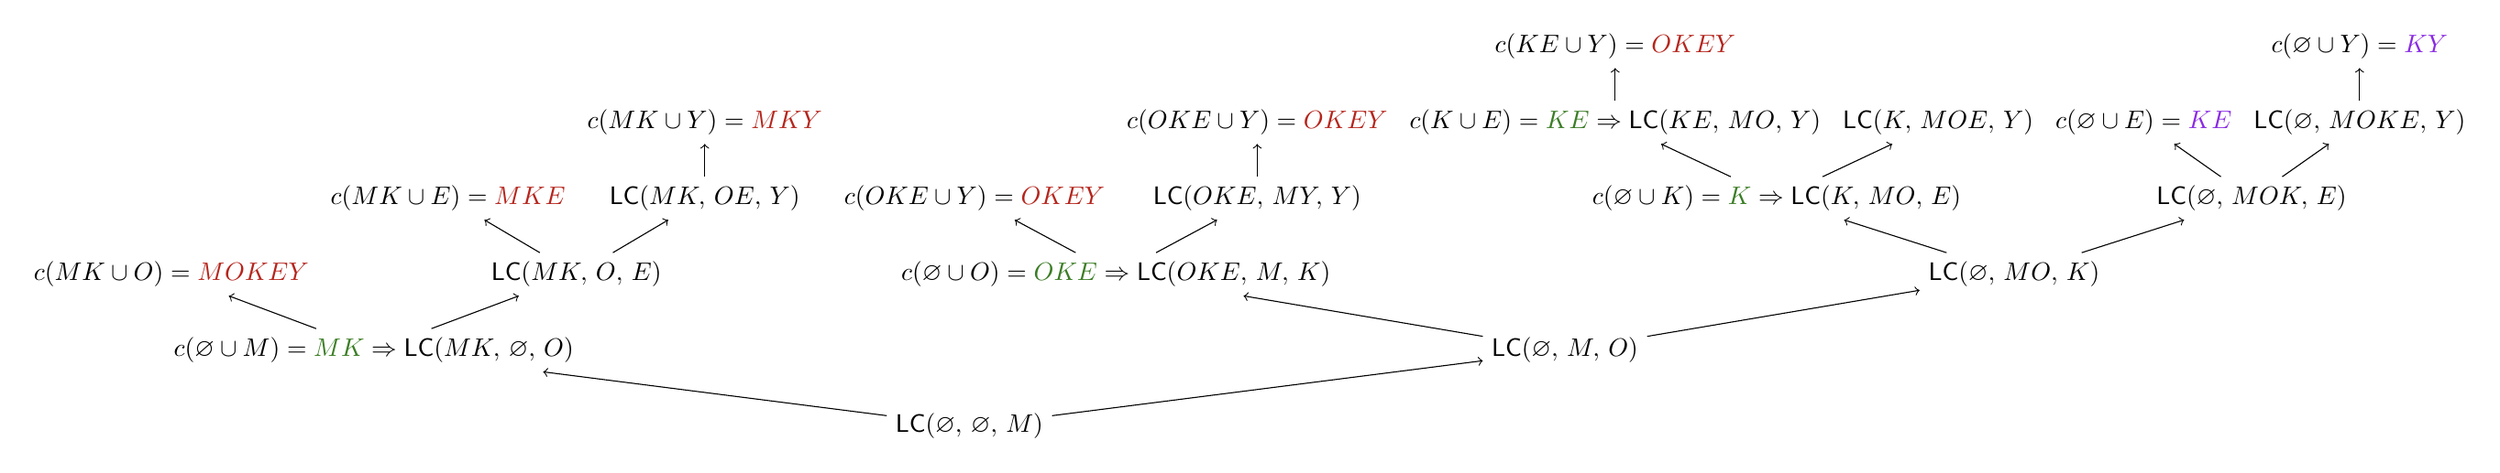
\begin{tikzpicture}[
      edge from parent/.style={draw, edge from parent path={(\tikzparentnode) -- (\tikzchildnode)}},
      edge from parent/.append style={->},
      grow'=up
    ]
      \Tree[. {$ \LC{\emptyset}{\emptyset}{M} $}
      [. {$c(\emptyset \cup M) = \frequent{MK} \Rightarrow \LC{MK}{\emptyset}{O} $}
        [. {$ c(MK \cup O) = \infrequent{MOKEY} $} ]
        [. {$ \LC{MK}{O}{E} $}
          [. {$ c(MK \cup E) = \infrequent{MKE} $} ]
          [. {$ \LC{MK}{OE}{Y} $}
            [. {$ c(MK \cup Y) = \infrequent{MKY} $} ]
          ]
        ]
      ]
      [. {$ \LC{\emptyset}{M}{O} $}
        [. {$c(\emptyset \cup O) = \frequent{OKE} \Rightarrow \LC{OKE}{M}{K} $}
          [. {$ c(OKE \cup Y) = \infrequent{OKEY} $} ]
          [. {$ \LC{OKE}{MY}{Y} $}
            [. {$ c(OKE \cup Y) = \infrequent{OKEY} $} ]
          ]
        ]
        [. {$ \LC{\emptyset}{MO}{K} $}
          [. {$c(\emptyset \cup K) = \frequent{K} \Rightarrow \LC{K}{MO}{E} $}
            [. {$c(K \cup E) = \frequent{KE} \Rightarrow \LC{KE}{MO}{Y} $}
              [. {$ c(KE \cup Y) = \infrequent{OKEY} $} ]
            ]
            [. {$ \LC{K}{MOE}{Y} $}
            ]
          ]
          [. {$ \LC{\emptyset}{MOK}{E} $}
            [. {$ c(\emptyset \cup E) = \intersects{KE} $} ]
            [. {$ \LC{\emptyset}{MOKE}{Y} $}
              [. {$ c(\emptyset \cup Y) = \intersects{KY} $} ]
            ]
          ]
        ]
      ]
    ]
    \end{tikzpicture}
  }

  As you can see from the tree%
  \footnote{It is small, but you can zoom in on the PDF. The tree is not an image and is fully rendered by \LaTeX!!},
  the algorithm outputs $\{MK,\, OKE,\, K,\, KE,\, KY\}$ which are our closed frequent itemsets.

  \subsection{Gély's algorithm proof}
  \begin{centerframebox}
    Prove the theorem on Slide 18 of 2023-11-22.

    \textbf{Theorem}:
    The previous algorithm lists the set of closed frequent itemsets
    \begin{enumerate}[label=(\arabic*)]
      \item correctly
      \item irredundantly
      \item with polynomial delay
      \item in polynomial space
    \end{enumerate}
  \end{centerframebox}
  \subsubsection{Soundness (Part of Correctness)}
  Before printing each itemset, the algorithm runs it through the closure operator $c()$ and checks whether or not it's frequent.
  And because $c()$ always returns a closed itemset, all the itemsets printed by the algorithm must be both closed and frequent.

  \subsubsection{Completeness (Part of Correctness)}
  TODO
  \subsubsection{Irredundancy}
  TODO
  \subsubsection{Polynomial delay}
  The main source of non-polynomial delay in the algorithm is the recursive call tree.
  But every time the it goes down the ``left'' branch (see Exercise 4.4) of the tree, it must print an itemset.
  So the maximum time that it can spend between printing two itemsets is the maximum amount of recursive steps it can take only going to the ``right'' branch of the tree.
  But since it only has one choice now, this number is no longer exponential and is limited by the maximum recursion depth $|I|$.

  \subsubsection{Polynomial space}
  The only space consuming structure this algorithm uses, if we exclude the input database, which is obviously takes up linear space,
  is the recursion stack.
  Each call to the $\LC{C}{N}{i}$ function need to store its own copy of $C$ and $N$ (and also $i$, but $i$ is just a number).
  Both $C$ and $N$ are itemsets, so their size is limited by $|I|$, which is part of the input database.
  And because on each recursive call the value of $i$ must increase by at least $1$, and it is limited to be an item from $I$,
  the maximum possible recursion depth is $|I|$.
  So the total space used for the stack is $2 \cdot |I|^2$, which is a polynomial on $|I|$.

  The closure computation might also need to store a copy of the database, but it is not recursive and we only have to count it once.
  Thus the total remains a polynomial.

\end{document}
